% ============================================================
%  PRISM — NeurIPS 2026 Anonymous Submission
%  Architecture details verified against codebase (2026-03).
% ============================================================
\documentclass{article}

% ── NeurIPS 2026 style (anonymous double-blind submission) ──
\usepackage{neurips_2026}

\usepackage[utf8]{inputenc}
\usepackage[T1]{fontenc}
\usepackage[colorlinks=true,linkcolor=blue,citecolor=blue,urlcolor=blue]{hyperref}
\usepackage{url}
\usepackage{booktabs}
\usepackage{amsmath}
\usepackage{amssymb}
\usepackage{amsfonts}
\usepackage{graphicx}
\usepackage{xcolor}
\usepackage{microtype}
\usepackage{nicefrac}
\usepackage{multirow}
\usepackage{subcaption}
\usepackage{enumitem}
\usepackage{colortbl}   % \rowcolor
\usepackage{makecell}   % \makecell for multi-line table cells
\usepackage{tikz}

% ── PRISM brand color ────────────────────────────────────────
\definecolor{prismblue}{RGB}{29, 78, 216}

% ── Custom macros ───────────────────────────────────────────
\newcommand{\Rbb}{\mathbb{R}}
\newcommand{\todo}[1]{\textcolor{red}{[\textbf{TODO:} #1]}}
\providecommand{\answerYes}[0]{\textcolor{green}{\textbf{Yes}}}
\providecommand{\answerNo}[0]{\textcolor{red}{\textbf{No}}}
\providecommand{\answerNA}[0]{\textcolor{gray}{\textbf{N/A}}}
\providecommand{\answerTODO}[0]{\textcolor{orange}{\textbf{TODO}}}
\providecommand{\justificationTODO}{\textcolor{orange}{\textit{TODO}}}

% ── Title ───────────────────────────────────────────────────
\title{\textcolor{prismblue}{PRISM}: Human \textcolor{prismblue}{P}oint Cloud \textcolor{prismblue}{R}econstruction v\textcolor{prismblue}{i}a \\
       \textcolor{prismblue}{S}keleton-Guided Diffusion from \textcolor{prismblue}{M}mWave Radar}

% TODO (camera-ready): fill in author names, affiliations, and emails.
\author{Anonymous Author(s)}

% ============================================================
\begin{document}
\maketitle

% ────────────────────────────────────────────────────────────
\begin{abstract}
Millimeter-wave~(mmWave) radar is an attractive modality for human sensing, offering
all-weather, non-contact, and privacy-preserving perception. However, its inherent sparsity severely limits downstream human-centric understanding, and there is currently no public dataset that provides paired quantitative benchmarks for dense human point cloud reconstruction under occlusion. We present MIST, the first mmWave human point
cloud dataset with paired quantitative benchmarks for
through-obstacle dense human reconstruction. MIST captures synchronized clear-view and through-obstacle observations of the same subjects performing identical actions, separated by a physical barrier, and provides LiDAR-based 3D ground truth. We further incorporate a three-level occlusion design that converts attenuation severity into a controlled variable, covering eight subjects, thirty action classes, and 640~k paired frames. To establish a baseline on MIST and address the limitations of point
cloud completion under extreme sparsity and human motion, we propose
PRISM, a skeleton-guided conditional latent diffusion framework for reconstructing dense human point clouds from sparse mmWave radar alone. Three conditioning streams—skeleton joint positions, coarse body geometry, and action class embeddings—are incorporated to guide a Dynamic Transformer within a VP-SDE framework, enabling effective denoising and the reconstruction of mmWave human point clouds with near-LiDAR quality. On MIST, PRISM achieves a COV-CD of 0.362, significantly outperforming the strongest completion baseline (0.113). Notably, PRISM maintains structurally coherent reconstruction even under severe through-obstacle attenuation at approximately 50 points per frame, whereas all baselines collapse to fixed-template outputs.
%Code and dataset are available at \url{https://mmwave-human.github.io/PRISM/}.
\end{abstract}

% ────────────────────────────────────────────────────────────
\section{Introduction}
\label{sec:intro}

% ── Teaser figure ───────────────────────────────────────────
\begin{figure}[t]
  \centering
  
\includegraphics[width=\linewidth, height=12cm, keepaspectratio]{assets/fig/teaser.jpg}
  \caption{
    Human point cloud quality across three sensing modalities under clear-view
    and through-obstacle conditions, illustrated with a forward kick action
    in which the kicking leg is partially occluded.
  }
  \label{fig:teaser}
\end{figure}

Millimeter-wave~(mmWave) radar has emerged as an increasingly attractive modality
for non-intrusive human sensing, operating reliably under complete darkness and
adverse weather without physical contact or line-of-sight
constraints~\cite{yang2023mm,zhang2023survey}.
These properties have enabled its adoption across a wide range of body-centric
tasks, including human activity recognition~\cite{huang2026ropehar,singh2019radhar,chang2025efficient},
skeletal pose estimation~\cite{wu2024mmhpe,ding2021radar,cao2024virteach,wang2025points},
and multi-person localization and tracking~\cite{feng2024m3pose}.
Its point cloud output carries no photorealistic record of the subject's
appearance, making it particularly well-suited for healthcare monitoring~\cite{liu2025contactless,wang2026remote} and
other privacy-sensitive scenarios~\cite{wang2026spectrogram}.

LiDAR and RGB-D cameras produce dense, geometrically accurate reconstructions
but cannot penetrate solid obstacles, making them unsuitable for through-wall
human monitoring. Although mmWave radar can penetrate non-metallic barriers, its point cloud density remains inherently limited by factors such as finite antenna aperture, bandwidth, signal-to-noise ratio, and the sparsity of human reflections, typically yielding only 50--150 points per frame. As Figure~\ref{fig:teaser} shows, occlusion further degrades mmWave point cloud
quality, while the kicking leg region disappears entirely from the LiDAR scan.
This combination of through-obstacle capability and inherent sparsity introduces a
dual challenge that remains unaddressed by existing datasets and methods.
All existing public mmWave human datasets~\cite{yang2023mm,an2022mri,fan2025m4human}
provide skeleton or mesh annotations while uniformly assuming unobstructed
sensor placement, while datasets that include an occlusion
scene~\cite{chen2022mmbody,zhao2018through} involves covering the sensor surface with
materials rather than placing a physical barrier between the sensor and subject,
precluding any simulation of real through-wall deployment and providing no
paired clear-view reference.
In terms of the approach, general-purpose point cloud completion
methods~\cite{yuan2018pcn,yu2021pointr,xiang2021snowflakenet} are designed for dense partial
observations of rigid synthetic objects and do not model the sequential
evolution of body geometry across an action.

We present MIST to enable systematic evaluation of through-obstacle mmWave human reconstruction by pairing clear-view and occluded observations under controlled barrier conditions, with synchronized LiDAR providing geometric supervision. To address reconstruction under such extreme sparsity, PRISM leverages radar-aligned joint representations inferred from sparse returns as structural priors within a conditional latent diffusion framework, guiding the denoising process toward temporally consistent and geometrically coherent human point clouds. As illustrated in Figure~\ref{fig:teaser}, PRISM reconstructs clear and structured
human point clouds under both clear-view and through-obstacle conditions,
faithfully recovering the kicking motion and approaching LiDAR reference
PRISM substantially outperforms raw mmWave input across three downstream
healthcare monitoring tasks, where activity recognition accuracy improves from 52.3\% to 73.1\%, pose estimation mean per joint position error (MPJPE) decreases from 138\,mm to 84\,mm,
and rehabilitation assessment correlation increases from 0.38 to 0.68. Our contributions are as follows:

\begin{itemize}[leftmargin=1.5em,itemsep=2pt]

  \item \textbf{MIST} is the first mmWave frequency-modulated continuous wave (FMCW) human point cloud dataset featuring a physical barrier between the sensor and the subject, providing paired clear-view and through-obstacle observations with synchronized overhead LiDAR as dense ground truth.
  A three-level occlusion design converts attenuation severity into a
  controlled experimental variable.
  MIST spans 8 subjects and 30 action classes, including rehabilitation and daily activities, with synchronized LiDAR, depth, and mmWave streams for multi-modal research.

  \item \textbf{PRISM} is a skeleton-guided conditional diffusion
  framework that reconstructs dense human point clouds from sparse mmWave
  radar. PRISM incorporates a skeleton keypoint detector SkelKD that first extracts radar-aligned joint positions before a Coarse Generator produces stable coarse body geometry
  robust to extreme input sparsity.
  Together with action class embeddings, these conditioning signals guide a
  Diffusion Denoiser under a denoising diffusion probabilistic model (DDPM) framework, constraining
  reconstruction to follow the kinematic evolution of each action.


  \item \textbf{Downstream task benchmarks.}
  Using the reconstructed sequences as input, we benchmarked PRISM against existing models on the MIST dataset for human action recognition, skeletal pose estimation, and rehabilitation
  exercise quality assessment.
  These benchmarks demonstrate that high-quality reconstruction yields
  substantial and consistent gains in performance across the full spectrum of body analysis
  required for real-world healthcare monitoring.

\end{itemize}

% ────────────────────────────────────────────────────────────
\section{Related work}
\label{sec:related}

\paragraph{mmWave-based human sensing datasets.}
Existing mmWave human datasets are collected under obstacle-free
conditions.
MM-Fi~\cite{yang2023mm} provides synchronized multi-modal streams and
M4Human~\cite{fan2025m4human} acquires high-fidelity mesh annotations via
marker-based motion capture, yet both datasets were collected in the absence of a physical barrier between
sensor and subject.
While mmBody~\cite{chen2022mmbody} includes an occlusion scene, the sensor surface is covered with materials with no paired clear-view reference and
no simulation of through-wall deployment.
This systematic gap leaves through-obstacle deployment without any quantitative benchmark.

\paragraph{Point cloud completion and human body reconstruction.}
Completion methods such as PCN~\cite{yuan2018pcn} and PoinTr~\cite{yu2021pointr} have been designed for dense partial scans of rigid synthetic objects\textemdash under the extreme sparsity and non-rigid articulation of human radar returns, their feature aggregation collapses to semantically empty representations. Generative models such as LION~\cite{vahdat2022lion} and LDT~\cite{ji2024latent} operate in
hierarchical variational autoencoder (VAE)~\cite{kingma2013auto} latent spaces with per-step conditioning for
expressive 3-D generation. However, both are conditioned on global latent codes or
dense spatial features extracted from the input rather than structured
anatomical priors. While mmPoint~\cite{xie2023mmpoint} recovers dense human point clouds from sparse
mmWave signals via deterministic regression, it generates a fixed
average-body template under extreme sparsity, leaving action categories
indistinguishable across frames. None of the above approaches incorporates joint-level skeletal topology as a
structural conditioning signal. In addition, these models are not designed for action-consistent
generation from streams of extremely sparse radar observations through
physical barriers.

\paragraph{Downstream task analysis.}
MiliPoint~\cite{cui2023milipoint} establishes action classification
benchmarks on sparse mmWave radar point clouds, and temporal methods such
as mmChainPose~\cite{lu2025mmchainpose} perform skeletal pose estimation by
propagating joint geometry cues across frames. Both approaches operate under obstacle-free sensor placement and evaluate on raw
radar returns rather than reconstructed dense clouds.
For rehabilitation exercise quality assessment, KIMORE~\cite{capecci2019kimore} offers kinematic scoring benchmarks derived from RGB-D sequences of
patients performing standardised exercises, demonstrating that precise
joint trajectory estimates translate to clinically meaningful motion
quality scores.
No existing benchmark evaluates activity recognition, pose estimation, or
rehabilitation exercise quality from point clouds reconstructed under
through-obstacle sensor conditions, leaving the downstream utility of
through-wall radar sensing without direct experimental validation.

% ────────────────────────────────────────────────────────────
\section{The MIST Dataset}
\label{sec:mist}
% ────────────────────────────────────────────────────────────

\begin{figure}[t]
  \centering
  
\includegraphics[width=\linewidth]{assets/fig/Dataset.jpg}
  \caption{
    Overview of MIST, comprising three occlusion levels, 30 action
    classes spanning rehabilitation and daily-living motions, and five
    sensing modalities providing ground truth.
  }
  \label{fig:mist_overview}
\end{figure}

All publicly available mmWave human datasets are collected under
obstacle-free conditions, leaving a critical evaluation gap for
through-obstacle deployment.
MIST addresses this by placing a physical barrier between the sensor and a subject, providing the first paired quantitative benchmark for
through-obstacle dense human point cloud reconstruction.
Three occlusion levels (OLs) are defined by the cumulative thickness of 18\,mm
wooden boards placed between the right-side radar and the subject, where
OL0 provides a clear line-of-sight without any boards, OL1 interposes one
18\,mm board, and OL2 stacks two boards to a total thickness of 36\,mm.
The 18\,mm board material matches the signal attenuation characteristics
of typical indoor partition materials while allowing reproducible,
incremental thickness control.
A detailed comparison with existing mmWave human datasets is provided
in Appendix~\ref{app:mist_compare}.

\paragraph{Sensor configuration.}
Two TI IWR6843 FMCW radars are mounted at $\sim$1.4\,m height,
one providing a clear-view path for OL0 capture and one operating through
the barrier at OL1 or OL2. Collecting both streams simultaneously
guarantees that every paired frame is captured at an identical subject pose.
An overhead Livox Mid-360 LiDAR and a door-side Intel RealSense D435i
depth camera (extrinsic-calibrated to a shared world coordinate frame) provide dense point clouds and 17-joint H36M skeleton ground truth~\cite{ionescu2013human3}.
Skeleton annotations are extracted at 30\,fps and resampled to 10\,fps
to match the radar frame rate.
Sensor specifications are listed in Appendix~\ref{app:mist_sensor}.

\paragraph{Occlusion levels and statistics.}
MIST defines three occlusion levels by cumulative board thickness.
OL0 provides 50--150 points per frame and serves as the primary training and evaluation split.
OL1, with a single board, attenuates signal returns to 25--80 points per frame,
and OL2 further reduces returns
to 10--30 points per frame due to signal attenuation from the two stacked boards.
The approximately five-fold density reduction from OL0 to OL2 causes FPS-based feature aggregation and all completion baselines to produce
degenerated outputs, making OL1 and OL2 a stress test for
density-invariant reconstruction. MIST covers eight subjects performing thirty action classes across three occlusion
levels with three repetitions per subject, yielding approximately 640 k
paired frames.

\paragraph{Action categories.}
The thirty action classes span two functional categories.
The rehabilitation category R01 to R14 covers fourteen classes targeting
upper and lower limb mobility, balance, and gait assessment relevant
to clinical motion screening.
The daily-living category D01 to D16 covers sixteen classes of whole-body
movements frequent in elderly-care monitoring, including D16 Forward
Fall, which directly supports fall detection as a downstream task.
Of the thirty classes, eight share equivalent kinematic categories with MM-Fi,
enabling direct cross-dataset transfer evaluation, and the complete action
list is provided in Appendix~\ref{app:mist_actions}.

\section{Method}
\label{sec:method}


% ── Full architecture figure ─────────────────────────────────
\begin{figure}[t]
  \centering
  
\includegraphics[width=\linewidth]{assets/fig/PRISM architecture overview.jpg}
  \caption{
    Overview of our proposed PRISM model, which consists of a skeleton alignment stage and a completion refinement stage. In the skeleton alignment stage, we extract and align multimodal features from LiDAR point clouds (dense), depth camera skeletons, and mmWave point clouds (sparse). These features serve as clean tokens and conditional information for the completion refinement stage. Notably, we design SkelKD and Temporal Adapter modules to respectively align skeleton predictions based on mmWave point clouds and fuse features across multiple time steps. In the completion refinement stage, we design a conditional DDPM equipped with clean tokens and conditional information from the previous stage to reconstruct enhanced point clouds, especially when the mmWave point clouds are partially occluded at test time.
  }
  \label{fig:arch}
\end{figure}

% ── Full architecture figure ─────────────────────────────────

% PRISM follows the two-path design in Figure~\ref{fig:arch}.
We propose PRISM, a novel skeleton-guided multimodal diffusion model, to verify the effectiveness and robustness of human point cloud reconstruction from mmWave radar based on our proposed MIST benchmark for healthcare downstream applications. 
During training, PRISM accepts multimodal inputs including mmWave, LiDAR, and deep camera, and learns a jointly aligned multimodal latent space for enhanced human point cloud reconstruction. At test time, our model achieves superior generalization using only mmWave input under various degrees of occlusion. 


\subsection{Skeleton Alignment}
\label{sec:overview}
As illustrated in Fig. \ref{fig:arch}, PRISM consists of two typical stages that skeleton alignment stage and completion refinement stage.
Skeleton alignment stage primary focus on extract, fuse and align multimodal features of input sequences from non-occluded LiDAR point clouds $\boldsymbol{x}_{\rm{lidar}} \in \mathbb{R}^{t \times m \times 3}$ and deep camera skeletons $\boldsymbol{x}_{\rm{deep}} \in \mathbb{R}^{t \times p \times 3}$, as well as partially-occluded mmWave point clouds $\boldsymbol{x}_{\rm{mmwave}} \in \mathbb{R}^{t \times n \times 3}$. Here $t$ denotes the number of frame in the point cloud sequence, $m$ and $n$ are the number of points per frame, and $p$ is the number of skeleton keypoints. In practice, we usually have $m > n \gg p$.
The temporal-fused LiDAR point cloud features, sampled under the guidance of deep camera skeletons, can be expressed as $\boldsymbol{h}_{\rm{lidar}}^{\rm{TA}}=f_{\boldsymbol{\theta}_{\rm{TA}}}(\boldsymbol{h}_{\rm{lidar}}^{\rm{PE}})$, $\boldsymbol{h}_{\rm{lidar}}^{\rm{PE}}=f_{\boldsymbol{\theta}_{\rm{PE}}}(\boldsymbol{x}_{\rm{lidar}}, \boldsymbol{x}_{\rm{deep}})$, where 
% $\boldsymbol{h}_{\rm{lidar}} \in \mathbb{R}^{t \times m \times d_{\rm{lidar}}}$, $d_{\rm{lidar}}$ is the feature dimension, 
$\boldsymbol{\theta}_{\rm{PE}}$ and $\boldsymbol{\theta}_{\rm{TA}}$ are separately denote the parameters of the PE Encoder \cite{yuan2018pcn} and our proposed Temporal Adapter module 
% (see details in Sec. \ref{sec:adapter}).
We propose SkelKD
(see details in Appendix~\ref{app:arch})
to predict skeleton keypoints $\boldsymbol{x}_{\rm{skelKD}} \in \mathbb{R}^{t \times p \times 3}$ from the pointwise features $\boldsymbol{h}_{\rm{mmwave}}^{\rm{point}}$ of mmWave point clouds $\boldsymbol{x}_{\rm{mmwave}}$. These features are extracted by a cascaded PCN Encoder \cite{kipf2016semi} followed by our proposed Temporal Adapter module as $\boldsymbol{x}_{\rm{skelKD}}=f_{\boldsymbol{\theta}_{\rm{seklKD}}}(\boldsymbol{h}_{\rm{mmwave}}^{\rm{point}})$, $\boldsymbol{h}_{\rm{mmwave}}^{\rm{point}}, \boldsymbol{h}_{\rm{mmwave}}^{\rm{global}}=f_{\boldsymbol{\theta}_{\rm{PCN}}}(\boldsymbol{x}_{\rm{mmwave}})$, where $\boldsymbol{\theta}_{\rm{skelKD}}$ and $\boldsymbol{\theta}_{\rm{PCN}}$ are parameters of PCN Encoder and our Temporal Adapter. Meanwhile, we use a graph convolutional network (GCN) Encoder \cite{tang2022lake} parameterized by $\boldsymbol{\theta}_{\rm{GCN}}$ to further aggregate the spatial information of the predicted skeleton keypoints $\boldsymbol{x}_{\rm{skelKD}}$, producing enhanced skeleton points $\boldsymbol{x}_{\rm{skelKD}}^{\rm{enhance}}=f_{\boldsymbol{\theta}_{\rm{GCN}}}(\boldsymbol{x}_{\rm{skelKD}})$ of the same shape as $\boldsymbol{x}_{\rm{skelKD}}$.
We then use a Coarse Generator \cite{kipf2016semi} to obtain the enhanced (dense but occluded) coarse point clouds given the concatenation of the pointwise features and global features, denoted by $\boldsymbol{x}_{\rm{mmwave}}^{\rm{dense}}=f_{\boldsymbol{\theta}_{\rm{CG}}}([\boldsymbol{h}_{\rm{mmwave}}^{\rm{point}}, \boldsymbol{h}_{\rm{mmwave}}^{\rm{global}}])$, where $\boldsymbol{\theta}_{\rm{CG}}$ is the parameters of Coarse Generator. 
Finally, the condition injection is constructed by putting action category $\boldsymbol{y}_{\rm{action}}$ like 'D03 Squat', the enhanced skeleton points $\boldsymbol{x}_{\rm{skelKD}}^{\rm{enhance}}$, and the enhanced coarse points $\boldsymbol{x}_{\rm{mmwave}}^{\rm{dense}}$ altogether.

\textbf{Temporal Adapter.}
Taking the Temporal Adapter applied on top of the PE encoder as an example (the same design is used for the Temporal Adapter after the PCN encoder). Specifically, we obtain temporally fused features $\boldsymbol{h}_{\rm{lidar}}^{\rm{TA}}$ by introducing a Transformer encoder layer parameterized by $\boldsymbol{\theta}_{\rm{TA}}$ on top of the frame-level features $\boldsymbol{h}_{\rm{lidar}}^{\rm{PE}} \in \mathbb{R}^{t \times q}$ from the PE Encoder, where $q = m \times d$ and $d$ is the feature dimension. Self-attention is applied along the temporal dimension~\cite{vaswani2017attention}.

\textbf{SkelKD.}
SkelKD regresses radar-aligned skeleton points $\boldsymbol{x}_{\rm{skelKD}}$ using PointNet \cite{qi2017pointnet}, a lightweight CNN-based feature extractor, from sparse mmWave point clouds $\boldsymbol{x}_{\rm{mmwave}}$ with deep camera supervision only. To avoid nearest-neighbor collapse under occlusion, SkelKD uses $p$ learnable joint query embeddings as cross-attention queries over per-point features extracted by a per-point MLP, with symmetric max-pooling over all $N$ returns yielding a global silhouette descriptor $\boldsymbol{h}_{\rm{global}}\!\in\!\mathbb{R}^{B\times256}$. Each query embedding attends over the full point set via scaled dot-product attention $\boldsymbol{f}_{\rm{joint}} = \mathrm{softmax}(QK^\top\!/\!\sqrt{d})\,V$ with $Q\!\in\!\mathbb{R}^{p\times128}$ and $K,V\!\in\!\mathbb{R}^{N\times128}$, so occluded joints spread their response across all visible returns rather than anchoring to a single noisy neighbor. The concatenated joint attention features and broadcast global descriptor are then mapped through a residual MLP regression head~\cite{he2016deep} to per-joint 3-D coordinates $\boldsymbol{x}_{\rm{skelKD}}\!\in\!\mathbb{R}^{t\times p\times3}$. 
% SkelKD is trained with $\mathcal{L}_{\rm{SkelKD}} = \mathcal{L}_{\rm{MPJPE}} + 0.1\,\mathcal{L}_{\rm{bone}}$, where $\mathcal{L}_{\rm{bone}}$ penalizes left-right bone-length asymmetry to enforce anatomical plausibility under partial observation. After Stage~1 pre-training, all SkelKD weights are frozen so that the diffusion stage trains against a stable skeleton representation, decoupled from denoiser co-adaptation.


\subsection{Completion Refinement}
% Completion Refinement phase in Fig. \ref{fig:arch} is mainly responsible for recover the non-occluded mmWave point clouds from their condition injection derived from the occluded and sparse mmWave point clouds. It contains a forward diffusion process that transferring the clean tokens from non-occluded and dense LiDAR point clouds into the noisy tokens and a backward diffusion process that denoising the noisy tokens with the conditional information extracted from mmWave point clouds.
The Completion Refinement phase in Fig. \ref{fig:arch} is mainly responsible for recovering clean point clouds from the conditional injection derived from occluded and sparse mmWave inputs. It consists of a forward diffusion process that progressively adds noise to clean tokens (obtained from non-occluded, dense LiDAR point clouds) to produce noisy tokens, and a backward diffusion process that denoises the noisy tokens using conditional information extracted from the mmWave point clouds.

\textbf{Forward Diffusion.}
Given the clean tokens of LiDAR point cloud features $\boldsymbol{z}_0 = \boldsymbol{h}_{\rm{lidar}}^{\rm{TA}}$, we apply the forward process of DDPM \cite{ho2020denoising,song2020score} to convert them into Gaussian noise $\boldsymbol{z}_T$ over $T$ time steps as:
\begin{align}
  q(\boldsymbol{z}_{1:T}|\boldsymbol{z}_0)=\prod_{t=1}^T q(\boldsymbol{z}_t|\boldsymbol{z}_{t-1}), \quad q(\boldsymbol{z}_t|\boldsymbol{z}_{t-1}) = \mathcal{N}(\sqrt{1-\beta_t} \boldsymbol{z}_{t-1}, \beta_t \textbf{I})
\end{align}
where $\beta_t$ is the noise level that typically set to be a small constant. The forward process 
% describing the relationship between $\boldsymbol{z}_t$ and $\boldsymbol{z}_0$ 
can be recursively derived as $q(\boldsymbol{z}_t|\boldsymbol{z}_0)=\mathcal{N}(\sqrt{\alpha_t} \boldsymbol{z}_0, (1-\alpha_t) \textbf{I})$, where $\alpha_t=\prod_{i=1}^{t} (1-\beta_i)$.

\textbf{Backward Diffusion.}
Given the condition injection $\boldsymbol{c}={\rm{EMB}}(\boldsymbol{y}_{\rm{action}}, \boldsymbol{x}_{\rm{skelKD}}^{\rm{enhance}}, \boldsymbol{x}_{\rm{mmwave}}^{\rm{dense}})$ derived from the embeddings of action category, skeleton points, and coarse points as illustrated in Fig. \ref{fig:arch}, we can gradually denoise from $\boldsymbol{z}_T$ conditioned on $\boldsymbol{c}$ as:
\begin{align}
  p_{\boldsymbol{\Theta}_{\rm{CR}}}(\boldsymbol{z}_{0:T}) = p_{\boldsymbol{\Theta}_{\rm{CR}}}(\boldsymbol{z}_{T}) \prod_{t=1}^{T} p_{\boldsymbol{\Theta}_{\rm{CR}}}(\boldsymbol{z}_{t-1}|\boldsymbol{z}_t),\ p_{\boldsymbol{\Theta}_{\rm{CR}}}(\boldsymbol{z}_{t-1}|\boldsymbol{z}_t) = \mathcal{N}(\boldsymbol{\mu}_{\boldsymbol{\Theta}_{\rm{CR}}}(\boldsymbol{z}_t, \boldsymbol{c}, t),\beta_t \textbf{I})
\end{align}
where $\boldsymbol{\Theta}_{\rm{CG}}$ are parameters of the conditional diffusion model in the Completion Refinement stage, $\boldsymbol{\mu}_{\boldsymbol{\Theta}_{\rm{CR}}}(\boldsymbol{z}_t, \boldsymbol{c}, t)=\frac{1}{\sqrt{1-\beta_t}}(\boldsymbol{z}_t - \frac{\beta_t}{\sqrt{1-\alpha_t}}\boldsymbol{\epsilon}_{\boldsymbol{\Theta}_{\rm{CR}}}(\boldsymbol{z}_t, \boldsymbol{c}, t))$.
The forward process provides ground truth signals for training the parameters in the backward process.

\begin{figure}[t]
  \centering
  
\includegraphics[width=0.75\linewidth]{assets/fig/MIST.jpg}
  \caption{
    MIST setup showing no board for OL0, one 18,mm board for OL1, and
    two 18,mm boards for OL2 are placed between the subject and the
    right-side mmWave radar, while the left-side LiDAR, mmWave radar, and
    depth camera remain unoccluded to provide ground truth.
  }
  \label{fig:mist_setup}
\end{figure}

\textbf{Training and Inference}:
We propose a skeleton-regularized noise prediction objective to train the model parameters $\boldsymbol{\Theta} = \{\boldsymbol{\Theta}_{\rm{SA}}, \boldsymbol{\Theta}_{\rm{CR}}\}$ as:
\begin{align} \label{eq:crmodel}
  \mathcal{L} = {\rm{min}}_{\boldsymbol{\Theta}} \mathbb{E}_{t,\boldsymbol{z}_0,\boldsymbol{\epsilon} \sim \mathcal{N}(\textbf{0}, \textbf{1})} \|\boldsymbol{\epsilon} - \boldsymbol{\epsilon}_{\boldsymbol{\Theta}_{\rm{CR}}}\|_2^2 + \lambda \|\boldsymbol{x}_{\rm{deep}} - \boldsymbol{x}_{\rm{skelKD}}\|_2^2
\end{align}
where $\boldsymbol{\Theta}_{\rm{SA}}=\{\boldsymbol{\theta}_{\rm{PE}}, \boldsymbol{\theta}_{\rm{TA}}, \boldsymbol{\theta}_{\rm{GCN}}, \boldsymbol{\theta}_{\rm{PCN}}, \boldsymbol{\theta}_{\rm{CG}}\}$ denote the parameters in Skeleton Alignment stage. The first term in Eq. \ref{eq:crmodel} aims to recover dense, non‑occluded human point clouds from sparse, partially occluded mmWave inputs. The second term aligns the skeletons predicted from mmWave point clouds with those from the depth camera.


% ────────────────────────────────────────────────────────────
\section{Experiments}
\label{sec:exp}
% ────────────────────────────────────────────────────────────

\subsection{Experiment Setup}
\label{sec:setup}
% ────────────────────────────────────────────────────────────

Data collection was performed within a controlled indoor laboratory with
approximately 5,m by 6,m usable floor area, as illustrated in
Figure~\ref{fig:mist_setup}.
Subjects performed all actions at 2 to 3,m from the sensor array.
The LiDAR, mmWave radar, and depth camera remained unoccluded
throughout, collecting complete unoccluded captures as dense reconstruction ground truth and ensuring that ground truth quality is unaffected by board placement. Three datasets OL0, OL1, and OL2 described in Section~\ref{sec:mist} and summarized in Table~\ref{tab:mist_compare} were collected. All sensors were extrinsically-calibrated to a shared world coordinate frame,
with calibration parameters held fixed across all subjects and sessions.

\paragraph{Training and evaluation protocol.}
Subjects P01 to P06 form the training split while P07 and P08 were held-out as evaluation split. All three occlusion levels were evaluated without obstacle-specific adaptation, providing a zero-shot test of density-invariant generalization. Training was performed on four sequential stages of SkelKD, Temporal Adapter, joint optimization of the Diffusion Denoiser with Condition Network and Coarse Generator,
and end-to-end fine-tuning via the Adam optimizer~\cite{kingma2014adam} with cosine learning-rate
decay. The full hyperparameters are listed in Appendix~\ref{app:training}. Cross-dataset generalization results, where all models are trained on
MIST and evaluated directly on MM-Fi~\cite{yang2023mm} using the
eight shared action classes, are reported in Appendix~\ref{app:mmfi_results}.


\subsection{Quantitative results on MIST}
\label{sec:quant}

\paragraph{Evaluation metrics.}
We adopt two set-level distribution metrics from~\cite{achlioptas2018learning}. In particular, COV-CD computes the fraction of ground-truth shapes matched by at least one
generated sample, rewarding broad coverage of the target distribution.
MMD-CD, on the other hand, determines the average distance from each ground-truth shape to its nearest
generated counterpart, rewarding distributional fidelity.
Results are reported per action and averaged over all thirty action classes.

\begin{table}[t]
  \centering
  \caption{
    Per-action point cloud quality on MIST-OL0
    (COV-CD$\uparrow$, MMD-CD$\downarrow$ scaled $\times10^{-3}$).
  }
  \label{tab:main}
  \footnotesize
  \setlength{\tabcolsep}{4pt}
  \resizebox{\linewidth}{!}{%
  \begin{tabular}{l l rr rr rr rr}
    \toprule
    \multirow{2}{*}{Method} & \multirow{2}{*}{Type}
      & \multicolumn{2}{c}{\textit{Squat}}
      & \multicolumn{2}{c}{\textit{Wave Hand}}
      & \multicolumn{2}{c}{\textit{Kick}}
      & \multicolumn{2}{c}{\textit{All}} \\
    \cmidrule(lr){3-4}\cmidrule(lr){5-6}\cmidrule(lr){7-8}\cmidrule(lr){9-10}
      & & COV & MMD & COV & MMD & COV & MMD & COV & MMD \\
    \midrule
    PCN~\cite{yuan2018pcn}                & Compl. & 0.079 & 9.16  & 0.088 & 8.92  & 0.082 & 9.04  & 0.083 & 9.01  \\
    PoinTr~\cite{yu2021pointr}          & Compl. & 0.108 & 8.37  & 0.121 & 8.14  & 0.114 & 8.25  & 0.113 & 8.26  \\
    SnowflakeNet~\cite{xiang2021snowflakenet} & Compl. & 0.071 & 10.86 & 0.083 & 10.61 & 0.076 & 10.74 & 0.079 & 10.72 \\
    LAKe-Net~\cite{tang2022lake}       & Compl. & 0.080 & 8.78  & 0.091 & 8.57  & 0.083 & 8.69  & 0.085 & 8.69  \\
    mmPoint~\cite{xie2023mmpoint}        & Det.   & 0.090 & 9.03  & 0.103 & 8.79  & 0.096 & 8.91  & 0.097 & 8.91  \\
    LION~\cite{vahdat2022lion}              & Gen.   & 0.173 & 7.49  & 0.192 & 7.27  & 0.183 & 7.38  & 0.185 & 7.37  \\
    TIGER~\cite{ren2024tiger}            & Gen.   & 0.197 & 7.21  & 0.219 & 6.97  & 0.209 & 7.11  & 0.209 & 7.08  \\
    \midrule
    PRISM (ours)                  & Gen.
      & 0.342 & 5.19
      & 0.392 & 4.62
      & 0.357 & 4.98
      & 0.362 & 4.83 \\
    \bottomrule
  \end{tabular}}
\end{table}

\paragraph{Results.}
Table~\ref{tab:main} shows that all seven baselines fail to generate action-discriminative reconstructions, though for different reasons. The four deterministic completion backbones cluster tightly between COV-CD 0.079
and 0.113, confirming that the ceiling is set by the absence of a body prior rather
than by model capacity.
SnowflakeNet underperforms PCN because its multi-stage farthest-point sampling
compounds density sensitivity at each upsampling level under extreme sparsity. mmPoint achieves COV-CD 0.097, barely above the completion cluster, because
single-frame deterministic regression cannot resolve pose ambiguity from a sparse,
action-agnostic radar input.
LION and TIGER fare noticeably better by sampling from a learned distribution,
achieving COV-CD 0.185 and 0.209, respectively.
Their remaining gap relative to PRISM reveals the limit of distribution diversity
without structural grounding, as the generated shapes cover the marginal body
distribution but are not steered toward any particular action.

PRISM achieves a COV-CD of 0.362 and an MMD-CD of $4.83\!\times\!10^{-3}$,
representing a $3.2\times$ improvement in coverage over PoinTr and a 41.5\%
reduction in matching distance, with consistent action discrimination across
Squat, Wave Hand, and Kick.
Qualitative visualisations of cross-action comparisons, temporal reconstruction, and the reverse diffusion process are provided in Appendix~\ref{app:qual}.


\subsection{Ablation study}
\label{sec:ablation}

% ── Ablation figure: COV-CD (blue) + MMD-CD (orange), two-metric layout ──
\begin{figure}[t]
\centering
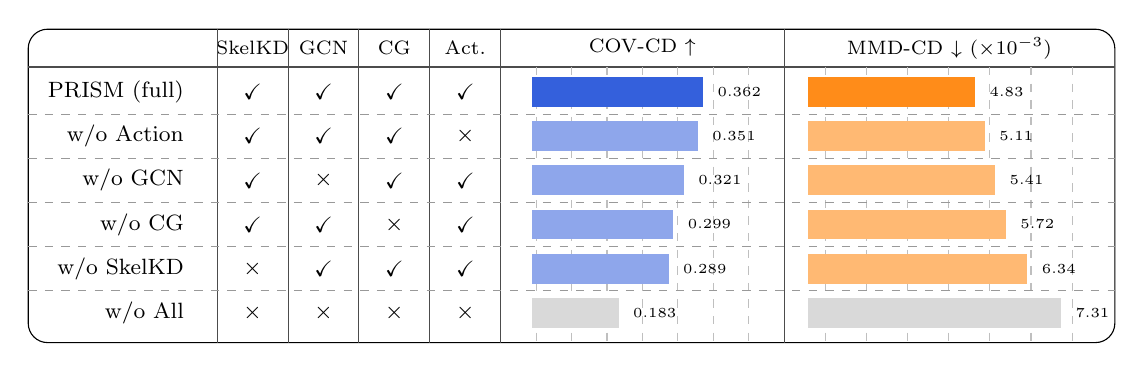
\begin{tikzpicture}[font=\footnotesize, x=1cm, y=1cm]

  %% ── Layout constants ────────────────────────────────────
  \def\rh{0.56}
  \def\bh{0.19}
  \def\xzero{-4.3}
  \def\xSK{-3.55}
  \def\xGC{-2.65}
  \def\xGA{-1.75}
  \def\xAC{-0.85}
  \def\xB{0.00}
  \def\xM{3.50}

  %% ── Precompute COV bar right-endpoints (start=0.00, scale=6.0) ──
  \pgfmathsetmacro{\cFull}{0.00+0.362*6.0}
  \pgfmathsetmacro{\cAct} {0.00+0.351*6.0}
  \pgfmathsetmacro{\cGCN} {0.00+0.321*6.0}
  \pgfmathsetmacro{\cGeo} {0.00+0.299*6.0}
  \pgfmathsetmacro{\cSkel}{0.00+0.289*6.0}
  \pgfmathsetmacro{\cAll} {0.00+0.183*6.0}

  %% ── Precompute MMD bar right-endpoints (start=3.50, scale=0.44) ──
  \pgfmathsetmacro{\mFull}{3.50+4.83*0.44}
  \pgfmathsetmacro{\mAct} {3.50+5.11*0.44}
  \pgfmathsetmacro{\mGCN} {3.50+5.41*0.44}
  \pgfmathsetmacro{\mGeo} {3.50+5.72*0.44}
  \pgfmathsetmacro{\mSkel}{3.50+6.34*0.44}
  \pgfmathsetmacro{\mAll} {3.50+7.31*0.44}

  %% ── Outer rounded-rectangle border ──────────────────────
  \draw[rounded corners=7pt, black, thin]
    (-6.40,-0.38) rectangle (7.40,3.60);

  %% ── Section headers ─────────────────────────────────────
  \node[font=\scriptsize] at (1.40,{5*\rh+0.56}) {COV-CD $\uparrow$};
  \node[font=\scriptsize] at (5.30,{5*\rh+0.56})
    {MMD-CD $\downarrow$ (${\times}10^{-3}$)};
  \node[align=center,font=\scriptsize] at (\xSK,{5*\rh+0.56}) {SkelKD};
  \node[align=center,font=\scriptsize] at (\xGC,{5*\rh+0.56}) {GCN};
  \node[align=center,font=\scriptsize] at (\xGA,{5*\rh+0.56}) {CG};
  \node[align=center,font=\scriptsize] at (\xAC,{5*\rh+0.56}) {Act.};

  %% ── Internal separators ──────────────────────────────────
  \draw[black!70,thin] (-6.40,{5*\rh+0.32}) -- (7.40,{5*\rh+0.32});
  \draw[black!70,thin] (-4.00,3.60) -- (-4.00,-0.38);
  \draw[black!70,thin] (-3.10,3.60) -- (-3.10,-0.38);
  \draw[black!70,thin] (-2.20,3.60) -- (-2.20,-0.38);
  \draw[black!70,thin] (-1.30,3.60) -- (-1.30,-0.38);
  \draw[black!70,thin] (-0.40,3.60) -- (-0.40,-0.38);
  \draw[black!70,thin] ( 3.20,3.60) -- ( 3.20,-0.38);

  %% ── Gridlines ────────────────────────────────────────────
  % COV area: -0.40 to 3.20, width=3.60, 7 inner lines at i/8, i=1..7
  % interval = 3.60/8 = 0.45
  \draw[black!25,thin,dashed] (0.05,{5*\rh+0.32})  -- (0.05,-0.38);   % 1/8
  \draw[black!25,thin,dashed] (0.50,{5*\rh+0.32})  -- (0.50,-0.38);   % 2/8
  \draw[black!25,thin,dashed] (0.95,{5*\rh+0.32})  -- (0.95,-0.38);   % 3/8
  \draw[black!25,thin,dashed] (1.40,{5*\rh+0.32})  -- (1.40,-0.38);   % 4/8
  \draw[black!25,thin,dashed] (1.85,{5*\rh+0.32})  -- (1.85,-0.38);   % 5/8
  \draw[black!25,thin,dashed] (2.30,{5*\rh+0.32})  -- (2.30,-0.38);   % 6/8
  \draw[black!25,thin,dashed] (2.75,{5*\rh+0.32})  -- (2.75,-0.38);   % 7/8

  % MMD area: 3.20 to 7.40, width=4.20, 7 inner lines at i/8, i=1..7
  % interval = 4.20/8 = 0.525
  \draw[black!25,thin,dashed] (3.7225,{5*\rh+0.32}) -- (3.7225,-0.38); % 1/8
  \draw[black!25,thin,dashed] (4.245,{5*\rh+0.32})  -- (4.245,-0.38);  % 2/8
  \draw[black!25,thin,dashed] (4.7675,{5*\rh+0.32}) -- (4.7675,-0.38); % 3/8
  \draw[black!25,thin,dashed] (5.290,{5*\rh+0.32})  -- (5.290,-0.38);  % 4/8
  \draw[black!25,thin,dashed] (5.8125,{5*\rh+0.32}) -- (5.8125,-0.38); % 5/8
  \draw[black!25,thin,dashed] (6.335,{5*\rh+0.32})  -- (6.335,-0.38);  % 6/8
  \draw[black!25,thin,dashed] (6.8575,{5*\rh+0.32}) -- (6.8575,-0.38); % 7/8

  % Row separators
  \draw[black!40,thin,dashed] (-6.40,{4.5*\rh}) -- (7.40,{4.5*\rh});
  \draw[black!40,thin,dashed] (-6.40,{3.5*\rh}) -- (7.40,{3.5*\rh});
  \draw[black!40,thin,dashed] (-6.40,{2.5*\rh}) -- (7.40,{2.5*\rh});
  \draw[black!40,thin,dashed] (-6.40,{1.5*\rh}) -- (7.40,{1.5*\rh});
  \draw[black!40,thin,dashed] (-6.40,{0.5*\rh}) -- (7.40,{0.5*\rh});

  %% ══════════════════════════════════════════════════════════
  %% Row 5 — PRISM (full)
  %% ══════════════════════════════════════════════════════════
  \node[anchor=east] at (\xzero,{5*\rh}) {PRISM (full)};
  \node at (\xSK,{5*\rh}) {\checkmark}; \node at (\xGC,{5*\rh}) {\checkmark};
  \node at (\xGA,{5*\rh}) {\checkmark}; \node at (\xAC,{5*\rh}) {\checkmark};
  \fill[prismblue!90] (\xB,{5*\rh-\bh}) rectangle (\cFull,{5*\rh+\bh});
  \node[anchor=west,font=\tiny] at (\cFull+0.06,{5*\rh}) {0.362};
  \fill[orange!90] (\xM,{5*\rh-\bh}) rectangle (\mFull,{5*\rh+\bh});
  \node[anchor=west,font=\tiny] at (\mFull+0.06,{5*\rh}) {4.83};

  %% ── Row 4 — w/o Action ──────────────────────────────────
  \node[anchor=east] at (\xzero,{4*\rh}) {w/o Action};
  \node at (\xSK,{4*\rh}) {\checkmark}; \node at (\xGC,{4*\rh}) {\checkmark};
  \node at (\xGA,{4*\rh}) {\checkmark}; \node at (\xAC,{4*\rh}) {$\times$};
  \fill[prismblue!50] (\xB,{4*\rh-\bh}) rectangle (\cAct,{4*\rh+\bh});
  \node[anchor=west,font=\tiny] at (\cAct+0.06,{4*\rh}) {0.351};
  \fill[orange!55] (\xM,{4*\rh-\bh}) rectangle (\mAct,{4*\rh+\bh});
  \node[anchor=west,font=\tiny] at (\mAct+0.06,{4*\rh}) {5.11};

  %% ── Row 3 — w/o GCN ─────────────────────────────────────
  \node[anchor=east] at (\xzero,{3*\rh}) {w/o GCN};
  \node at (\xSK,{3*\rh}) {\checkmark}; \node at (\xGC,{3*\rh}) {$\times$};
  \node at (\xGA,{3*\rh}) {\checkmark}; \node at (\xAC,{3*\rh}) {\checkmark};
  \fill[prismblue!50] (\xB,{3*\rh-\bh}) rectangle (\cGCN,{3*\rh+\bh});
  \node[anchor=west,font=\tiny] at (\cGCN+0.06,{3*\rh}) {0.321};
  \fill[orange!55] (\xM,{3*\rh-\bh}) rectangle (\mGCN,{3*\rh+\bh});
  \node[anchor=west,font=\tiny] at (\mGCN+0.06,{3*\rh}) {5.41};

  %% ── Row 2 — w/o CG ─────────────────────────────────────
  \node[anchor=east] at (\xzero,{2*\rh}) {w/o CG};
  \node at (\xSK,{2*\rh}) {\checkmark}; \node at (\xGC,{2*\rh}) {\checkmark};
  \node at (\xGA,{2*\rh}) {$\times$};   \node at (\xAC,{2*\rh}) {\checkmark};
  \fill[prismblue!50] (\xB,{2*\rh-\bh}) rectangle (\cGeo,{2*\rh+\bh});
  \node[anchor=west,font=\tiny] at (\cGeo+0.06,{2*\rh}) {0.299};
  \fill[orange!55] (\xM,{2*\rh-\bh}) rectangle (\mGeo,{2*\rh+\bh});
  \node[anchor=west,font=\tiny] at (\mGeo+0.06,{2*\rh}) {5.72};

  %% ── Row 1 — w/o SkelKD ──────────────────────────────────
  \node[anchor=east] at (\xzero,{1*\rh}) {w/o SkelKD};
  \node at (\xSK,{1*\rh}) {$\times$};   \node at (\xGC,{1*\rh}) {\checkmark};
  \node at (\xGA,{1*\rh}) {\checkmark}; \node at (\xAC,{1*\rh}) {\checkmark};
  \fill[prismblue!50] (\xB,{1*\rh-\bh}) rectangle (\cSkel,{1*\rh+\bh});
  \node[anchor=west,font=\tiny] at (\cSkel+0.06,{1*\rh}) {0.289};
  \fill[orange!55] (\xM,{1*\rh-\bh}) rectangle (\mSkel,{1*\rh+\bh});
  \node[anchor=west,font=\tiny] at (\mSkel+0.06,{1*\rh}) {6.34};

  %% ── Row 0 — w/o All ─────────────────────────────────────
  \node[anchor=east] at (\xzero,{0*\rh}) {w/o All};
  \node at (\xSK,{0*\rh}) {$\times$}; \node at (\xGC,{0*\rh}) {$\times$};
  \node at (\xGA,{0*\rh}) {$\times$}; \node at (\xAC,{0*\rh}) {$\times$};
  \fill[gray!30] (\xB,{0*\rh-\bh}) rectangle (\cAll,{0*\rh+\bh});
  \node[anchor=west,font=\tiny] at (\cAll+0.06,{0*\rh}) {0.183};
  \fill[gray!30] (\xM,{0*\rh-\bh}) rectangle (\mAll,{0*\rh+\bh});
  \node[anchor=west,font=\tiny] at (\mAll+0.06,{0*\rh}) {7.31};

\end{tikzpicture}
\caption{
  Component ablation on MIST-OL0.
  COV-CD and MMD-CD for each conditioning module.
}
\label{fig:ablation}
\end{figure}


Figure~\ref{fig:ablation} reports the contribution of each conditioning module
on the MIST-OL0 validation split.
SkelKD is the dominant component, as its removal drops COV-CD from 0.362 to 0.289
and raises MMD-CD to 6.34, the largest single-module degradation.
The Coarse Generator and GCN each contribute meaningfully, reducing COV-CD to 0.299 and 0.321
respectively when removed, confirming that stable coarse geometry and kinematic-chain
propagation are both necessary for full-body coverage.
The action label has the smallest individual effect yet remains relevant for actions
sharing similar instantaneous joint configurations.
Removing all three streams collapses COV-CD to 0.183, on par with unconditional LION,
isolating the gains to the conditioning stack rather than the diffusion backbone.
Through-obstacle robustness on OL1 and OL2 is reported in Appendix~\ref{app:mist_eval}.


\subsection{Downstream task evaluation}
\label{sec:downstream}

We evaluate downstream utility across three tasks using a shared PointNet++
backbone~\cite{qi2017pointnet,qi2017pointnetpp} with lightweight task-specific heads,
comparing raw mmWave input against PoinTr, TIGER, and PRISM across OL0 to OL2.
Figure~\ref{fig:radar} summarises performance on five evaluation axes: HAR
accuracy at OL0, fall detection F1, pose estimation quality, rehabilitation
assessment correlation, and robustness at OL2.
An unoccluded LiDAR oracle forms the outer ring as the modality upper bound.
PRISM leads all reconstruction baselines on every axis, and the advantage over
raw mmWave widens consistently as occlusion severity increases.

\begin{figure}[t]
  \centering
  \begin{minipage}[b]{0.52\linewidth}
    \centering
    
\includegraphics[width=\linewidth]{assets/fig/downstream_radar.jpg}
    \caption{Downstream task performance radar chart across five axes.
      LiDAR Oracle (grey) defines the outer ring.}
    \label{fig:radar}
  \end{minipage}
  \hfill
  \begin{minipage}[b]{0.45\linewidth}
    \centering
    
\includegraphics[width=\linewidth]{assets/fig/tsne_action.jpg}
    \caption{t-SNE of action features on 16 daily-living classes.
      (a)~Raw mmWave input and (b)~PRISM reconstruction.}
    \label{fig:tsne}
  \end{minipage}
\end{figure}

\paragraph{Human activity recognition.}
We use the 16 daily-living action classes in MIST for this evaluation.
PRISM reaches 73.1\% top-1 accuracy at OL0, which is 20.8 percentage
points above raw mmWave and 5.9 points above TIGER.
Under heavy occlusion at OL2 the margin widens to 24.1 percentage points,
showing that reconstruction disproportionately benefits harder sensing conditions.
The t-SNE visualization in Figure~\ref{fig:tsne} corroborates this at the feature
level, where raw mmWave roughly separates broad action groups but still confuses similar
motion types such as lower-body activities, while PRISM reconstructions form
tighter and more separable clusters despite residual coupling between adjacent
classes.

\paragraph{Human pose estimation.}
A 17-joint regression head predicts H36M-convention joint coordinates, with
accuracy measured in MPJPE, and full results appear in Table~\ref{tab:downstream}.
PRISM reduces MPJPE from 138\,mm to 84\,mm at OL0 and still achieves 112\,mm
at OL2, which remains below raw mmWave at clear-view OL0, demonstrating that
reconstruction compensates effectively for through-obstacle signal attenuation.
The MPJPE gap between PRISM and raw mmWave grows from 54\,mm at OL0 to 79\,mm
at OL2.

\paragraph{Rehabilitation exercise quality assessment.}
Motion quality scores derived from per-joint velocity cosine similarity for classes
R01--R14 are compared with LiDAR reference scores by Pearson correlation,
with detailed results in Table~\ref{tab:downstream}.
PRISM achieves $r\!=\!0.68$ at OL0, surpassing raw mmWave at $r\!=\!0.38$ and
PoinTr at $r\!=\!0.51$.
At OL2, PRISM retains $r\!=\!0.53$ while raw mmWave drops to $r\!=\!0.24$,
confirming that PRISM supports clinically meaningful exercise monitoring without
requiring unobstructed sensor placement.

\begin{table}[t]
  \centering
  \caption{Downstream task performance on MIST (test subjects P07--P08).}
  \label{tab:downstream}
  \tiny
  \setlength{\tabcolsep}{4pt}
  \resizebox{\linewidth}{!}{%
  \begin{tabular}{l ccc c ccc ccc}
    \toprule
    & \multicolumn{3}{c}{HAR Acc (\%)$\uparrow$}
    & \multirow{2}{*}{\makecell{Fall\\F1$\uparrow$}}
    & \multicolumn{3}{c}{HPE MPJPE (mm)$\downarrow$}
    & \multicolumn{3}{c}{Rehab $r$$\uparrow$} \\
    \cmidrule(lr){2-4}\cmidrule(lr){6-8}\cmidrule(lr){9-11}
    Input & OL0 & OL1 & OL2 & & OL0 & OL1 & OL2 & OL0 & OL1 & OL2 \\
    \midrule
    Raw mmWave
      & 52.3 & 43.6 & 35.2 & 0.628
      & 138  & 163  & 191
      & 0.38 & 0.31 & 0.24 \\
    PoinTr~\cite{yu2021pointr}
      & 63.8 & 57.1 & 49.4 & 0.741
      & 116  & 147  & 172
      & 0.51 & 0.44 & 0.37 \\
    TIGER~\cite{ren2024tiger}
      & 67.2 & 60.1 & 53.8 & 0.782
      & 104  & 131  & 158
      & 0.58 & 0.51 & 0.43 \\
    PRISM (ours)
      & \textbf{73.1} & \textbf{66.8} & \textbf{59.3} & \textbf{0.851}
      & \textbf{84}   & \textbf{96}   & \textbf{112}
      & \textbf{0.68} & \textbf{0.61} & \textbf{0.53} \\
    \bottomrule
  \end{tabular}}
\end{table}


% ────────────────────────────────────────────────────────────
\section{Limitations}
\label{sec:limitations}

MIST was collected using 18\,mm wooden boards as the sole barrier material, and reconstruction quality under barriers with substantially different electromagnetic properties, such as metal, reinforced concrete, or laminated glass, remains uncharacterized.
The dataset covers eight subjects from a single controlled laboratory, and the participant pool does not span a wide range of body morphologies or age groups, which may limit cross-population generalization to individuals whose physiology differs substantially from those in the training set.
At inference time, PRISM requires 200 reverse diffusion steps, resulting in per-frame latency exceeding 1\,s on a single GPU, and accelerating this through consistency distillation or flow-matching reparameterization is a natural direction for future work.
Both MIST and PRISM assume a single subject within the sensing volume, and extending through-obstacle reconstruction to multi-person scenes with overlapping radar returns requires new conditioning strategies and a substantially revised data collection protocol.

% ────────────────────────────────────────────────────────────
\section{Conclusion}
\label{sec:conclusion}

We presented MIST, the first through-obstacle mmWave human benchmark with three
paired occlusion levels and synchronized LiDAR ground truth, and PRISM, a
skeleton-guided latent diffusion framework that reconstructs dense human point
clouds from sparse mmWave radar alone.
PRISM resolves the two failure modes of prior approaches by inferring radar-aligned
skeleton joints from sparse returns, pairing them with density-invariant coarse
geometry and action embeddings, and injecting this structural prior at every
denoising step of a latent diffusion model.
On MIST, PRISM achieves COV-CD 0.362 against 0.113 for the strongest completion
baseline and maintains action-discriminative reconstruction at OL2 where all
deterministic baselines collapse, and downstream evaluations confirm that PRISM
reconstructions consistently outperform raw mmWave at every occlusion level, with
OL2 outputs still surpassing raw mmWave under clear-view conditions.
Together, MIST and PRISM provide a foundation for privacy-preserving,
through-obstacle healthcare monitoring using mmWave radar alone.

% ────────────────────────────────────────────────────────────
\begin{ack}
% Hidden in anonymous submission; fill before camera-ready.
\todo{Acknowledgments and funding disclosure. Do NOT include in anonymized submission.}
\end{ack}

% ────────────────────────────────────────────────────────────
\bibliographystyle{unsrt}
\bibliography{references}


% ============================================================
%  Appendix  (unlimited pages; does NOT count toward page limit)
% ============================================================

\appendix

% ============================================================
\section{MIST dataset details}
\label{app:mist}
% ============================================================

\subsection{Comparison with Existing mmWave Datasets}
\label{app:mist_compare}

Table~\ref{tab:mist_compare} compares representative mmWave human sensing datasets along
five axes, where \emph{Phys.\ Barrier} indicates a physical object between sensor and subject,
\emph{Paired} indicates simultaneous clear-view and occluded captures of identical poses,
\emph{LiDAR GT} indicates synchronized overhead LiDAR as dense 3-D reconstruction ground truth,
\emph{Skel/Mesh GT} indicates skeleton or mesh annotations, and \emph{OL} indicates the
number of controlled occlusion levels.
RF-Pose uses sub-6\,GHz radio and produces 2-D skeleton heatmaps rather than a point cloud,
and mmBody's occlusion variant covers the sensor aperture rather than placing a physical barrier
between sensor and subject.

\paragraph{Obstacle-free benchmarks.}
The dominant paradigm collects data under clear sensor--subject line-of-sight.
mmMesh~\cite{xue2021mmmesh} pioneered human mesh construction from sparse 60\,GHz
reflections but covered only 20 subjects across 8 actions with no occlusion scenario.
mmBody~\cite{chen2022mmbody} expanded action coverage to 100 categories with paired mesh
annotations, and its occlusion variant places absorbent material over the sensor aperture
rather than a physical barrier, providing no spatial selectivity and no clear-view reference.
mRI~\cite{an2022mri} pairs mmWave with RGB-D and inertial sensing for 3-D skeleton
annotation under obstacle-free conditions.
MM-Fi~\cite{yang2023mm} includes synchronized overhead LiDAR as a dense reconstruction
reference but collects every session in an open indoor space without any barrier.
M4Human~\cite{fan2025m4human} scales to 50 action categories with Vicon mesh annotations
yet retains the same obstacle-free assumption.

\paragraph{Through-barrier and simulated-occlusion sensing.}
RF-Pose~\cite{zhao2018through} demonstrated that a physical wall need not block human sensing, using
sub-6\,GHz radio signals to produce 2-D skeleton heatmaps of subjects behind a wall.
However, the sub-60\,GHz frequency band, 2-D output format, single fixed wall, and absence
of a simultaneous clear-view reference or LiDAR reconstruction target leave mmWave-specific
dense point cloud reconstruction under controlled multi-level occlusion unaddressed.

\paragraph{MIST.}
MIST is the first mmWave dataset to simultaneously satisfy all three requirements.
Occlusion levels are defined by cumulative board thickness, where OL0 uses no board,
OL1 interposes one 18\,mm wooden board, and OL2 stacks two boards totalling 36\,mm between
the subject and one radar, and a second co-located radar maintains an unobstructed path, so
every frame provides a paired clear-view capture at OL0 and through-obstacle captures at OL1
and OL2 of the identical pose.
An overhead Livox Mid-360 LiDAR, physically separated from the barrier, provides dense
reconstruction ground truth unaffected by board placement across all levels.
The three-level occlusion design converts attenuation severity into a controlled experimental
variable, enabling the first direct evaluation of density-invariant reconstruction under
realistic through-barrier conditions.

\begin{table}[h]
  \centering
  \caption{Comparison of MIST with representative mmWave human sensing datasets.}
  \label{tab:mist_compare}
  \footnotesize
  \setlength{\tabcolsep}{3.5pt}
  \resizebox{\linewidth}{!}{%
  \begin{tabular}{lcccccccccc}
    \toprule
    \multirow{2}{*}{Dataset} & \multirow{2}{*}{Year}
      & \multirow{2}{*}{\makecell{Phys.\\Barrier}}
      & \multirow{2}{*}{Paired}
      & \multirow{2}{*}{\makecell{LiDAR\\GT}}
      & \multirow{2}{*}{\makecell{Skel/Mesh\\GT}}
      & \multirow{2}{*}{OL}
      & \multirow{2}{*}{\#Subj}
      & \multirow{2}{*}{\#Act}
      & \multirow{2}{*}{\#Frames}
      & \multirow{2}{*}{\makecell{mmWave\\pts/frame}} \\
    \\
    \midrule
    RF-Pose~\cite{zhao2018through}         & 2018 & \checkmark           & \texttimes & \texttimes & \texttimes           & 1 & $\sim$100 & 1   & --           & -- \\
    mmMesh~\cite{xue2021mmmesh}          & 2021 & \texttimes           & \texttimes & \texttimes & \checkmark\ (mesh)   & 1 & 20        & 8   & $\sim$3k     & $\sim$50 \\
    mmBody~\cite{chen2022mmbody}          & 2022 & \texttimes           & \texttimes & \texttimes & \checkmark\ (mesh)   & 1 & 20        & 100 & $\sim$200k   & $\sim$200 \\
    mRI~\cite{an2022mri}                & 2022 & \texttimes           & \texttimes & \texttimes & \checkmark\ (skel)   & 1 & 20        & 12  & $\sim$160k   & 50--150 \\
    MM-Fi~\cite{yang2023mm}     & 2023 & \texttimes           & \texttimes & \checkmark & \checkmark\ (skel)   & 1 & 40        & 27  & $>$320k      & 50--150 \\
    M4Human~\cite{fan2025m4human}        & 2024 & \texttimes           & \texttimes & \texttimes & \checkmark\ (mesh)   & 1 & 20        & 50  & $\sim$661k   & 50--150 \\
    \midrule
    MIST (ours) & 2026
      & \checkmark & \checkmark & \checkmark & \checkmark\ (skel)
      & 3 & 8 & 30 & $\sim$640k
      & \makecell{50--150 (OL0)\\25--80 (OL1)\\10--30 (OL2)} \\
    \bottomrule
  \end{tabular}}
\end{table}

\subsection{Sensor Configuration}
\label{app:mist_sensor}

Data collection took place in a controlled indoor laboratory with approximately
5\,m $\times$ 6\,m usable floor area, where subjects performed actions at 2--3\,m
from the door-side sensor array.
Two TI IWR6843 FMCW radars are co-located at $\sim$1.4\,m, one
maintaining a clear line-of-sight for OL0 and one operating through a wooden
barrier of 18\,mm for OL1 or two stacked boards totalling 36\,mm for OL2,
and collecting both streams simultaneously ensures that every paired frame is
captured at an identical subject pose.
A Livox Mid-360 LiDAR is mounted overhead and extrinsic-calibrated to a shared
world coordinate frame, providing 360° dense point clouds as reconstruction
ground truth unaffected by board placement.
An Intel RealSense D435i depth camera at the door-side mount delivers
synchronized RGB-D streams from which H36M-17 skeleton ground truth is
extracted at 30\,fps and resampled to 10\,fps to match the radar frame rate.
Table~\ref{tab:mist_sensor} summarises the key sensor parameters.

\begin{table}[h]
  \centering
  \caption{
    MIST sensor specifications.
    N/A indicates the parameter is not applicable to that modality.
  }
  \label{tab:mist_sensor}
  \small
  \setlength{\tabcolsep}{4pt}
  \resizebox{\linewidth}{!}{%
  \begin{tabular}{llll}
    \toprule
    Parameter            & TI IWR6843 $\times$2          & Livox Mid-360                        & Intel RealSense D435i \\
    \midrule
    Modality             & 60--64\,GHz FMCW              & 905\,nm LiDAR                        & RGB-D and IMU \\
    Bandwidth            & 4\,GHz                        & N/A                                  & N/A \\
    Range resolution     & 4.4\,cm                       & 2\,cm                                & N/A \\
    Max range            & 5\,m                          & 40\,m                                & 0.1--10\,m \\
    Velocity resolution  & 0.13\,m/s                     & N/A                                  & N/A \\
    Field of view        & $\pm60°$ az and $\pm15°$ el   & $360°$ az and $-7°$ to $52°$ el      & $87°\times58°$ \\
    Antenna              & 3\,Tx $\times$ 4\,Rx          & N/A                                  & N/A \\
    Frame rate           & 10\,fps                       & 10\,fps                              & 30\,fps \\
    Color and depth res. & N/A                           & N/A                                  & 640$\times$480 \\
    Skeleton convention  & N/A                           & N/A                                  & H36M-17 joints \\
    \bottomrule
  \end{tabular}}
\end{table}

\subsection{Action List}
\label{app:mist_actions}

MIST covers 30 action classes across two functional categories.
The rehabilitation category includes 14 exercises targeting upper and lower limb
mobility, balance, and gait assessment relevant to clinical motion screening.
The daily-living category includes 16 activities emphasising whole-body movements
that appear frequently in elderly-care monitoring scenarios.
Of the 30 actions, 8 share equivalent kinematic categories with MM-Fi, enabling direct cross-dataset transfer evaluation.

\begin{table}[h]
  \centering
  \caption{MIST complete action list.}
  \label{tab:mist_actions}
  \small
  \setlength{\tabcolsep}{4pt}
  \resizebox{\linewidth}{!}{%
  \begin{tabular}{cl cl cl cl}
    \toprule
    \multicolumn{4}{c}{\textit{Rehabilitation (R01--R14)}} &
    \multicolumn{4}{c}{\textit{Daily Living (D01--D16)}} \\
    \cmidrule(r){1-4}\cmidrule(l){5-8}
    R01 & Shoulder forward flexion & R08 & Knee extension       & D01 & Standing still        & D09 & Reaching overhead \\
    R02 & Shoulder abduction       & R09 & Ankle dorsiflexion   & D02 & Walking in place      & D10 & Full body turn \\
    R03 & Elbow flexion extension  & R10 & Balance left leg     & D03 & Squat                 & D11 & Waving hand \\
    R04 & Bilateral wrist rotation & R11 & Balance right leg    & D04 & Rising from chair     & D12 & Phone call gesture \\
    R05 & Neck rotation            & R12 & Tandem gait          & D05 & Raising arms overhead & D13 & Clapping \\
    R06 & Trunk side bend          & R13 & Sit to stand         & D06 & Forward bend          & D14 & Forward kick \\
    R07 & Hip flexion              & R14 & Lateral weight shift & D07 & Picking up object     & D15 & Jumping in place \\
         &                         &     &                      & D08 & Carrying object       & D16 & Forward fall \\
    \bottomrule
  \end{tabular}}
\end{table}

\subsection{Directory Structure}

Figure~\ref{fig:mist_dir} shows the hierarchical layout of the MIST dataset.
The root contains one sub-directory per subject (S01--S08), and each subject
directory is further divided by action (A01--A30, corresponding to R01--R14 and
D01--D16).
Within each action folder, the paired occlusion design is reflected directly in
the directory structure, where one sub-folder pairs OL0 (clear-view) with OL1
(18\,mm board), and a second sub-folder pairs OL0 with OL2 (36\,mm total),
so that every through-obstacle capture has an exact simultaneous clear-view
counterpart at the same pose.
Each occlusion-level folder stores five synchronized modalities: mmWave radar
point clouds (\texttt{.npy}), LiDAR point clouds (\texttt{.bin}), depth maps
(\texttt{.npy}), RGB frames (\texttt{.png}), and a single per-sequence skeleton
annotation file (\texttt{ground\_truth\_h36m.npy}) providing 17-joint H36M
coordinates at 10\,fps.

\begin{figure}[h]
  \centering
  \includegraphics[width=0.85\linewidth]{assets/fig/The expanded directory.jpg}
  \caption{Expanded directory structure of the MIST dataset.}
  \label{fig:mist_dir}
\end{figure}

% ============================================================
\section{Architecture and training details}
\label{app:arch}
% ============================================================

\begin{figure}[t]
  \centering
  
\includegraphics[width=\linewidth]{assets/fig/SkelKD.jpg}
  \caption{
    SkelKD architecture in which 17 learnable joint query embeddings attend over
    encoded radar returns via cross-attention to regress radar-aligned skeleton joints.
  }
  \label{fig:skelkd}
\end{figure}

\subsection{Module Hyperparameters}

Table~\ref{tab:arch} lists the architecture hyperparameters for each PRISM
module.
All hidden dimensions, attention head counts, and layer depths are chosen to
balance expressive capacity with training feasibility on
three NVIDIA A6000 GPUs (48\,GB each).
The Temporal Adapter output dimension of $8\times120$ is fixed prior to diffusion
training and shared across all conditioning configurations. The structure of SkelKD is shown in ~\ref{fig:skelkd}

\begin{table}[h]
  \centering
  \caption{
    PRISM module hyperparameters.
  }
  \label{tab:arch}
  \small
  \setlength{\tabcolsep}{6pt}
  \begin{tabular}{lll}
    \toprule
    Module & Parameter & Value \\
    \midrule
    \multirow{3}{*}{SkelKD}
      & Conv feature dim (local)        & 128 \\
      & Global pooled feature dim       & 256 \\
      & Joint query embeddings          & $17\times128$ \\
    \midrule
    \multirow{4}{*}{Temporal Adapter}
      & Transformer encoder layers      & 6 \\
      & Output feature dim              & 20 ($8\times120$ total) \\
      & Hidden dim and attention heads  & 128 and 4 \\
      & Output tokens $K$               & 256 \\
    \midrule
    \multirow{2}{*}{Coarse Generator}
      & Feature dim                     & 256 \\
      & Output coarse points            & 128 \\
    \midrule
    \multirow{3}{*}{Condition Network}
      & GCN layers and node dim         & 2 and 256 \\
      & Coarse-geometry encoder         & Conv1d, 256 channels \\
      & Total K/V tokens                & 145 (17 skeleton + 128 geometry) \\
    \midrule
    \multirow{3}{*}{Diffusion Denoiser}
      & Residual blocks                 & 6 \\
      & Hidden dim and attention heads  & 256 and 4 \\
      & Conditioning                    & AdaLN~\cite{ba2016layer} and CFG~\cite{ho2022classifier} \\
    \bottomrule
  \end{tabular}
\end{table}

\subsection{Training Schedule}
\label{app:training}

PRISM is trained in four sequential stages on three NVIDIA A6000 GPUs (48\,GB each).
Stage~1 pre-trains SkelKD at a learning rate of $10^{-3}$ with batch size 16 for
5000 epochs (approximately 12\,h) and freezes it.
Stage~2 trains the Temporal Adapter independently at $2\!\times\!10^{-4}$ with batch size 8
for 3000 epochs (approximately 48\,h) and freezes it.
Stage~3 jointly optimises the Diffusion Denoiser, Condition Network, and Coarse Generator
at $2\!\times\!10^{-4}$ with batch size 16 for 5000 epochs
(approximately 24\,h).
Stage~4 fine-tunes all components except SkelKD end-to-end at $3\!\times\!10^{-5}$
with batch size 16 for 2000 epochs (approximately 8\,h).
All stages use Adam with cosine learning-rate decay, gradient clipping at 1.0, and 500 warm-up steps,
and Stages~3 and~4 additionally apply EMA with decay 0.9999.

% ============================================================
\section{Additional experiments}
\label{app:additional}
% ============================================================

\subsection{Cross-dataset generalization on MM-Fi}
\label{app:mmfi_results}

To evaluate cross-dataset generalisation, all models are trained on MIST-OL0 and
evaluated directly on MM-Fi~\cite{yang2023mm}, a large-scale public benchmark
comprising 40 subjects performing 27 action classes across 4 environments with
synchronised mmWave point clouds and depth-camera skeleton ground truth under the
H36M convention.
Evaluation covers the 8 action classes shared between MIST and MM-Fi, namely A03,
A12, A13, A17, A19, A22, A26, and A27, using test subjects S08 to S10 from
environment E01.
Baseline methods are additionally re-trained on MM-Fi subjects S01 to S07 to
provide an in-domain upper bound, while PRISM transfers directly from its MIST-trained
weights without any MM-Fi-specific fine-tuning.

Table~\ref{tab:mmfi_appendix} shows that PRISM achieves consistent improvements
on MM-Fi comparable to those on MIST-OL0.
MMD-CD is 40.6\% lower than the best completion baseline PoinTr and COV-CD is
220\% higher, confirming that skeleton-guided conditioning transfers across dataset
conditions without any target-domain fine-tuning.
The 1-NN-CD gap between PRISM and LION narrows compared to MIST, which is expected, given that with 7 training subjects in MM-Fi versus 6 in MIST-OL0, unconditional generative
baselines benefit from a richer training distribution, while PRISM's skeleton conditioning
still provides the decisive structural advantage.
The SnowflakeNet degradation, with COV-CD 0.081 falling below PCN at 0.086,
replicates the pattern observed on MIST, confirming that multi-stage farthest-point
sampling failure under extreme sparsity is an architectural limitation rather than a
dataset artefact.

\begin{table}[h]
  \centering
  \caption{Cross-dataset generalization on MM-Fi across 8 overlapping action classes on test subjects S08 to S10. Methods marked $^*$ are re-trained on MM-Fi, while PRISM transfers directly from MIST-trained weights without fine-tuning.}
  \label{tab:mmfi_appendix}
  \small
  \setlength{\tabcolsep}{5pt}
  \begin{tabular}{llcccc}
    \toprule
    Method & Venue & Type
           & MMD-CD$\downarrow$ & COV-CD$\uparrow$ & 1-NN-CD$\downarrow$ \\
    \midrule
    PCN$^*$~\cite{yuan2018pcn}               & 3DV'18     & Compl. & 0.00887 & 0.0855 & 0.9994 \\
    PoinTr$^*$~\cite{yu2021pointr}         & ICCV'21    & Compl. & 0.00813 & 0.1172 & 0.9989 \\
    SnowflakeNet$^*$~\cite{xiang2021snowflakenet}& ICCV'21    & Compl. & 0.01056 & 0.0808 & 0.9998 \\
    LAKe-Net$^*$~\cite{tang2022lake}      & CVPR'22    & Compl. & 0.00856 & 0.0878 & 0.9993 \\
    mmPoint$^*$~\cite{xie2023mmpoint}       & BMVC'23    & Det.   & 0.00877 & 0.0991 & 0.9995 \\
    LION$^*$~\cite{vahdat2022lion}             & NeurIPS'22 & Gen.   & 0.00724 & 0.1892 & 0.9813 \\
    TIGER$^*$~\cite{ren2024tiger}           & CVPR'24    & Gen.   & 0.00695 & 0.2147 & 0.9776 \\
    \midrule
    PRISM (ours)                     & --         & Gen.   & 0.00483 & 0.3748 & 0.9697 \\
    \bottomrule
  \end{tabular}
\end{table}

Per-action COV-CD on MM-Fi ranges from 0.344 for Arm Raise, which involves subtle
distal motion, to 0.412 for Bowing, which involves pronounced full-body displacement,
with a macro-average of 0.374 consistent with the aggregate in Table~\ref{tab:mmfi_appendix},
confirming that per-frame skeleton conditioning is the primary driver of action-level
discrimination.

\subsection{Through-obstacle robustness on OL1 and OL2}
\label{app:mist_eval}

Table~\ref{tab:mist_per_level} disaggregates the through-obstacle evaluation
by occlusion level, complementing the main-text discussion of OL1/OL2 robustness.
All methods are trained exclusively on MIST-OL0 (P01--P06) and evaluated
zero-shot on OL1 and OL2 with no obstacle-specific adaptation.

At OL1, where a single 18\,mm board attenuates returns to 25--80 points per frame,
PRISM retains a COV-CD of 0.298, a relative drop of 17.7\% from OL0, while all
deterministic baselines drop to COV-CD below 0.07, a relative degradation of
40--50\%.
At OL2, where two stacked 18\,mm boards totalling 36\,mm reduce returns to 10--30 points
per frame, the most severe condition in MIST, PRISM still achieves
a COV-CD of 0.214 while baselines collapse below 0.035.
The $\Delta$COV columns confirm that PRISM's relative degradation is consistently
two to three times smaller than any baseline across both occlusion levels.

Two design choices jointly account for this resilience.
First, the Coarse Generator maps inputs of any density to 128 stable coarse body points,
so geometric anchoring remains intact even when FPS-based aggregation degenerates
under extreme sparsity.
Second, SkelKD's cross-attention aggregation spreads over all visible returns
rather than relying on a nearest-neighbor match, so the skeleton conditioning signal
degrades gracefully as the return count falls rather than producing a catastrophic
feature collapse.
Together, these properties allow PRISM to maintain action-discriminative
reconstruction at point densities where every deterministic baseline produces a
fixed-template output.


\begin{table}[h]
  \centering
  \caption{Through-obstacle robustness on MIST (zero-shot from OL0 training). $\Delta$COV: relative COV-CD change from OL0, COV/MMD: COV-CD/MMD-CD.}
  \label{tab:mist_per_level}
  \small
  \setlength{\tabcolsep}{3.5pt}
  \begin{tabular}{ll cccc cccc}
    \toprule
    & & \multicolumn{4}{c}{OL1} & \multicolumn{4}{c}{OL2} \\
    \cmidrule(r){3-6}\cmidrule(l){7-10}
    Method & Type
      & MMD$\downarrow$ & COV$\uparrow$ & 1-NN$\downarrow$ & $\Delta$COV
      & MMD$\downarrow$ & COV$\uparrow$ & 1-NN$\downarrow$ & $\Delta$COV \\
    \midrule
    PCN$^*$~\cite{yuan2018pcn}
      & Compl. & 0.0142 & 0.051 & 0.9961 & $-38.6\%$
               & 0.0182 & 0.021 & 0.9983 & $-74.7\%$ \\
    PoinTr$^*$~\cite{yu2021pointr}
      & Compl. & 0.0126 & 0.067 & 0.9949 & $-40.9\%$
               & 0.0166 & 0.031 & 0.9973 & $-72.6\%$ \\
    SnowflakeNet$^*$~\cite{xiang2021snowflakenet}
      & Compl. & 0.0183 & 0.039 & 0.9972 & $-50.6\%$
               & 0.0225 & 0.017 & 0.9990 & $-78.5\%$ \\
    mmPoint$^*$~\cite{xie2023mmpoint}
      & Det.   & 0.0151 & 0.054 & 0.9957 & $-44.3\%$
               & 0.0191 & 0.024 & 0.9979 & $-75.2\%$ \\
    PRISM (ours)
      & Gen.   & 0.0076 & 0.298 & 0.9734 & $-17.7\%$
               & 0.0102 & 0.214 & 0.9768 & $-40.9\%$ \\
    \bottomrule
  \end{tabular}
\end{table}

% ============================================================
\section{Qualitative results}
\label{app:qual}
% ============================================================

\subsection{Cross-action comparison}
\label{app:qual_main}

\begin{figure}[h]
  \centering
  
\includegraphics[width=\linewidth]{assets/fig/qual_comparison.jpg}
  \caption{
    Cross-action qualitative comparison of four actions (rows) versus six methods
    (columns), with LiDAR ground truth as the rightmost column.
  }
  \label{fig:qual}
\end{figure}




Figure~\ref{fig:qual} illustrates the two dominant failure modes of baseline methods.
For distal limb actions such as Wave Hand and Kick, all baselines produce a neutral
standing shape regardless of pose, as the sparse radar returns from a raised arm or
swinging leg are insufficient to activate the nearest-neighbour features that
completion backbones rely on, and unconditional generative methods lack the structural
prior needed to distinguish these configurations from rest.
Squat exposes a different failure mode, as the full-body postural change distributes
returns across an unusual spatial extent, causing baselines to average over the
observed cloud and yield a blurred, anatomically inconsistent shape.
Per-frame skeleton conditioning steers PRISM toward the correct kinematic state in
all four actions, producing body shapes that faithfully match the LiDAR ground truth
silhouette and limb arrangement.

\begin{figure}[h]
  \centering
  
\includegraphics[width=\linewidth]{assets/fig/diffusion_grid.jpg}
  \caption{
    VP-SDE reverse denoising process for action D06 Forward Bend, subject P01,
    visualised at six timesteps from $t\!=\!1.0$ to $t\!=\!0$.
  }
  \label{fig:diffusion_process}
\end{figure}

\begin{figure}[h]
  \centering
  
\includegraphics[width=\linewidth, height=12cm, keepaspectratio]{assets/fig/temporal_bow.jpg}
  \caption{
    Temporal point cloud reconstruction across three timesteps of a bowing
    sequence, comparing baseline methods and PRISM against LiDAR ground truth.
  }
  \label{fig:temporal_bow}
\end{figure}


\subsection{Latent diffusion process}
\label{app:diffusion}

Figure~\ref{fig:diffusion_process} visualises the step-by-step reverse process
in the Temporal Adapter feature space for a single bowing frame.
Each panel shows the decoded point cloud at a fixed denoising timestep, from
pure noise at $t\!=\!1.0$ on the left to the fully denoised output at $t\!=\!0$
on the right.
Starting from isotropic Gaussian noise, the Diffusion Denoiser
progressively resolves global body structure before refining local pose detail.
This coarse-to-fine behaviour is consistent across all 30 MIST action classes.
Actions with large limb displacements establish recognisable global body structure as early as
$t\!=\!0.6$, as the skeleton K/V tokens inject a strong kinematic prior at every
denoising layer.
Actions with subtle distal motion maintain the correct global silhouette from
$t\!=\!0.6$ but require later timesteps to resolve fine-grained limb configurations.

\subsection{Temporal reconstruction across a bowing sequence}
\label{app:teaser}

Figure~\ref{fig:temporal_bow} compares point cloud reconstruction across three
timesteps of a bowing sequence, from an upright starting pose through mid-bow
to the fully extended bow.
All four baselines produce a near-identical upright silhouette at every timestep
regardless of the pronounced trunk flexion between frames, as completion backbones
trained on rigid objects have no mechanism to track continuous non-rigid articulation
and unconditional generative models converge to the marginal body distribution
independent of the sparse radar input.
PRISM faithfully tracks the bow arc at each step, progressively deepening the
trunk angle while maintaining anatomically plausible limb geometry, because the
radar-aligned skeleton joints injected as conditioning tokens at every denoising
step anchor the reconstruction to the current kinematic state of the subject.
This temporal fidelity emerges from per-frame conditioning alone and requires no
explicit across-frame sequence modelling.




% ────────────────────────────────────────────────────────────
% NeurIPS 2026 mandatory checklist (does NOT count toward page limit)
% ────────────────────────────────────────────────────────────
\newpage
\input{checklist}


\end{document}